% xjupiter-c3-server-s2ss-c2-4.tex

\documentclass{standalone}
% jupiter-illustration-preamble.tex

\usepackage{tikz}
\usetikzlibrary{shapes, positioning, arrows.meta, calc, backgrounds, fit}

\def\hdist{1.8}
\def\vdist{2.0}
\tikzset{node distance = \vdist and \hdist}

\tikzset{every lower node part/.style = {red}}
\newcommand{\statesplit}[4]{% #1: state upper label; #2: state lower label; #3: position; #4
  \node (#4) [circle split, draw, minimum size = 6mm, text width = 10mm, align = center, #3, font = \Large]
  {
	$#1$
	\nodepart{lower}
	$#2$
  };
}

\newcommand{\transition}[4][]{% #2: start state; #3: end state; #4: transition label; #1: transition label position (optional)
  \draw[>=Stealth, ->] (#2) to node (#2to#3) [rectangle, draw, above = 2pt, sloped, #1, font = \small] {$#4$} (#3);
}

\newcommand{\set}[1]{\{#1\}}
\newcommand{\ins}[2]{\textsc{Ins}(#1,#2)}
\newcommand{\del}[2]{\textsc{Del}(#1,#2)}


\begin{document}
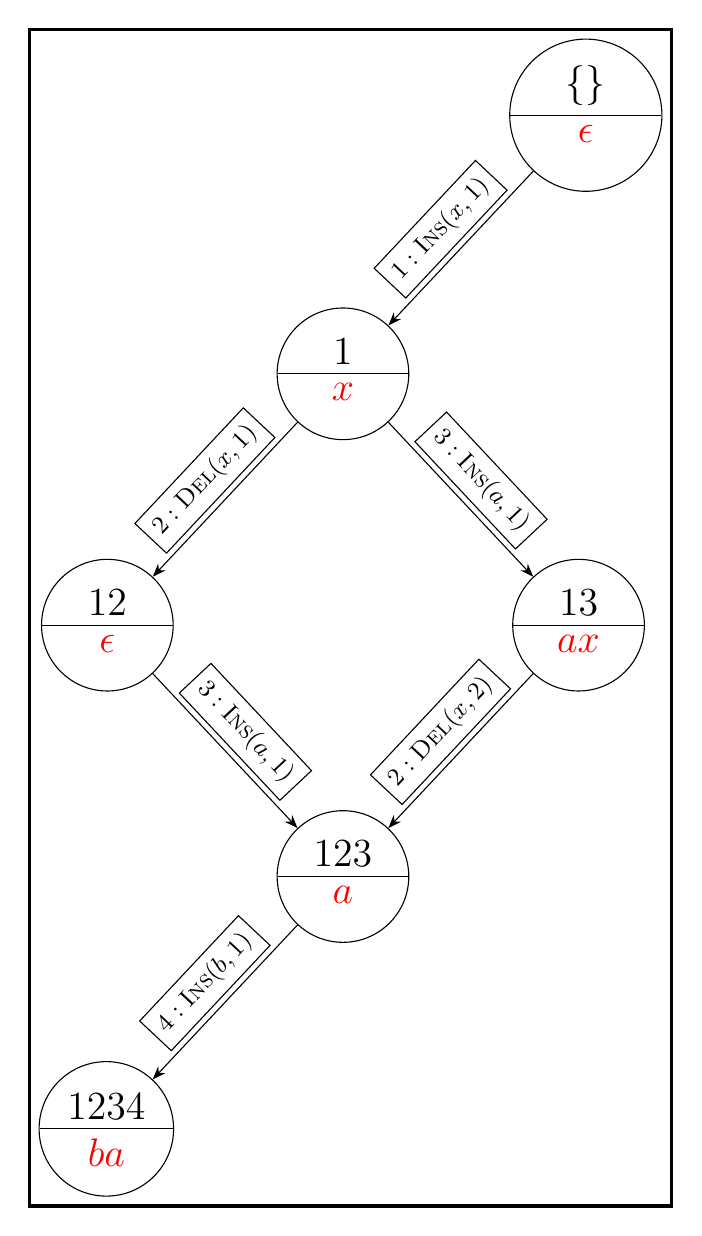
\begin{tikzpicture}[bg/.style = {rectangle, draw, very thick}]
  \statesplit{\{\}}{\epsilon}{}{0}

  \statesplit{1}{x}{below left = of 0}{1}
  \transition{0}{1}{1: \ins{x}{1}}

  \statesplit{12}{\epsilon}{below left = of 1}{12}
  \transition{1}{12}{2: \del{x}{1}}

  \statesplit{13}{ax}{below right = of 1}{13}
  \transition{1}{13}{3: \ins{a}{1}}

  \statesplit{123}{a}{below right = of 12}{123}
  \transition{12}{123}{3: \ins{a}{1}}
  \transition{13}{123}{2: \del{x}{2}}

  \statesplit{1234}{ba}{below left = of 123}{1234}
  \transition{123}{1234}{4: \ins{b}{1}}

  \node () [fit = (0) (1) (12) (13) (123) (1234), bg] {};
\end{tikzpicture}
\end{document}